\chapter{Perancangan}
\label{chap:perancangan}

Berdasarkan analisis yang telah dilakukan, terdapat beberapa hal yang perlu dirancang untuk pembangunan perangkat lunak sederhana analisis waktu tempuh kota Bandung ini. Pada bab ini akan dijelaskan mengenai perancangan aplikasi yang akan dibangun meliputi perancangan file keluaran, perancangan antarmuka, kelas diagram kelas rinci beserta deskripsi dan fungsinya.

\section{Kebutuhan Masukan dan Keluaran}
\label{sec:kebutuhaninputoutput}

Perangkat lunak yang dibangun merupakan perangkat lunak untuk melakukan ekstraksi data dari layanan Google Direction. Pada perancangan perangkat lunak ini menggunakan \textit{library} jsoup untuk melalukan \textit{request} ke layanan Google Direction. Selain itu perangkat lunak ini akan menggunakan \textit{library} JSON untuk mengekstraksi \textit{output} JSON yang merupakan \textit{response} dari \textit{request} yang diminta. Masukan dan keluaran perangkat lunak adalah sebagai berikut :

\subsection{Masukan}
\label{subsec:input}

Masukan dari perangkat lunak sederhana ini adalah parameter-parameter yang digunakan untuk melakukan request. Parameter-parameter tersebut adalah : \textit{origin, departure\_time} dalam bentuk unix, dan \textit{traffic\_model}. Nilai parameter \textit{origin} adalah nilai \textit{longitude} dan \textit{latitude} yang disatukan menjadi sebuah string. \textit{Longitude} dan \textit{latitude} itu sendiri adalah \textit{longitude} dan \textit{latitude} dari masing-masing sample. Nilai parameter \textit{departure\_time} adalah nilai unix yang di-\textit{parsing} menjadi bentuk string dari sebuah tanggal. Nilai parameter \textit{traffic\_model} adalah sebuah string salah satu dari \textit{best\_guess, optimistic, pessimistic}.

\subsection{Keluaran}
\label{subsec:output}

Keluaran dari perangkat lunak sederhana ini adalah sebuah file dengan ekstensi \textit{Comma Separated Value} (.csv) dimana dalam file ini berisi data hasil ekstraksi dari \textit{request} ke layanan Google Direction.

\section{Parameter \textit{request} ke layanan Google Direction}
\label{sec:parameterrequest}

Sesuai dengan subbab \ref{sec:analisisrequestgoogledir}, \textit{request} berbentuk sebuah url dengan memasukan parameter-parameter yang dibutuhkan keladam url untuk melakukan suatu \textit{request}. Nilai dari parameter \textit{origin} yang akan digunakan pada perangkat lunak ini dibagi menjadi 2 yaitu : sampel 1 dengan nilai "`-6.9536001,107.6193958"' dan sampel 2 dengan nilai "`-6.937021,107.6643817"'. Nilai dari parameter \textit{destination} yang akan digunakan pada perangkat lunak ini adalah "`-6.8746025,107.6024968"' yang merupakan nilai \textit{longitude} dan \textit{latitude} dari Universitas Katolik Parahyangan. 

\section{Rancangan file keluaran}
\label{sec:rancanganfile}

Sesuai dengan subsubbab \ref{subsec:output}, data pada file ini memiliki format tersusun dari nilai-nilai yang dipisahkan oleh koma(,). Menggunakan aplikasi Microsoft Excel, setiap nilai-nilai yang dipisahkan oleh koma(,) ini di direpresentasikan dengan masing-masing kolom. Sesuai masukan dari pengguna, file keluaran ini sendiri terbagi menjadi tiga tergantung dari \textit{traffic\_model} yang dipilih. Berikut ini merupakan tiga macam keluaran yang akan dihasilkan oleh perangkat lunak sederhana ini :

\begin{itemize}
	\item file ekstensi .csv dengan tiga nilai : file ini akan dihasilkan jika pengguna memilih satu \textit{traffic\_model} dimana nilai pertama adalah nilai yang merepresentasikan hari, nilai kedua adalah nilai merepresentasikan jam dan nilai yang terakhir adalah nilai waktu tempuh sesuai dengan yang dipilih oleh pengguna.
	\item file ekstensi .csv dengan empat nilai : file ini akan dihasilkan jika pengguna memilih dua \textit{traffic\_model} dimana nilai pertama adalah nilai yang merepresentasikan hari, nilai kedua adalah nilai merepresentasikan jam, nilai yang ketiga dan keempat adalah nilai waktu tempuh sesuai dengan yang dipilih oleh pengguna. Kombinasi pilihan pengguna yang memungkinkan adalah \textit{best\_guess} dan \textit{optimistic}, \textit{best\_guess} dan \textit{pessimistic}, \textit{optimistic} dan \textit{pessimistic}. 
	\item file ekstensi .csv dengan lima nilai : file ini akan dihasilkan jika pengguna memilih satu \textit{traffic\_model} dimana nilai pertama adalah nilai yang merepresentasikan hari, nilai kedua adalah nilai merepresentasikan jam, nilai ketiga, keempat dan kelima adalah nilai waktu tempuh sesuai dengan yang dipilih oleh pengguna dengan kombinasi pilihan pengguna adalah \textit{best\_guess}, \textit{optimisic} dan \textit{pessimistic}.
\end{itemize}

\section{Diagram Kelas Rinci}
\label{sec:diagramkelasrinci}

Diagram kelas rinci diperoleh dari hasil pengembangan diagram kelas analisis pada subbab \ref{sec:analisisclassdiagram}. Diagram kelas rinci dapat dilihat pada Gambar \ref{fig:kelasdiagramrinci}. Deskripsi kelas beserta fungsi dari diagram kelas rinci tersebut adalah sebagai berikut:
\begin{enumerate}
	\item DurationIntrafficExtractor
	
	Kelas ini merupakan kelas yang bertugas untuk melakukan \textit{request} ke Google Direction API dan mengekstraksi nilai waktu dalam satuan detik dari \textit{response} balasan dari \textit{request} yang diminta. Kelas ini melakukan satu \textit{request} dalam satu waktu. Kelas ini juga melakukan penghitungan konversi dari nilai waktu yang bersatuan detik menjadi menit. Atribut yang dimiliki oleh kelas ini antara lain :
	
	\begin{itemize}
		\item \textbf{private String DIRECTION\_URL :} merupakan url dasar untuk melakukan \textit{request} ke Google Direction API.
		\item \textbf{private String APIKEY :} merupakan sebuah kunci API yang akan dimasukan kedalam url dasar sebagai salah satu parameter untuk dapat melacak penggunaannya.
		\item \textbf{private String LANGUAGE :} merupakan salah satu parameter untuk url dasar yang berfungsi untuk memberikan \textit{response} dari Google Direction dalam suatu bahasa.
		\item \textbf{private String departureTime :} merupakan salah satu parameter untuk url dasar untuk menentukan waktu keberangkatan dari suatu titik ke tempat tujuan.
		\item \textbf{private String origin :} merupakan parameter wajib untuk url dasar yang merepresentasikan suatu titik berupa \textit{longitude} dan \textit{latitude} dari suatu tempat yang dijadikan acuan dasar tempat keberangkatan ke tempat tujuan.
		\item \textbf{private String destination :} merupakan parameter wajib untuk url dasar yang merepresentasikan suatu titik berupa \textit{longitude} dan \textit{latitude} dari suatu tempat yang dijadikan acuan dasar tempat tujuan.
		\item \textbf{private int time :} merupakan sebuah attribut yang berisikan waktu dalam hitungan menit yang didapatkan dari hasil ekstraksi \textit{response} \textbf{duration\_in\_traffic} dari suatu \textit{request}. 
	\end{itemize}
	
	Method-method yang dimiliki kelas ini merupakan action method dengan rincian sebagai berikut:
	
	\begin{itemize}
		\item \textbf{public DurationInTrafficExtractor(String unix, String origin, String destination, String trafficModel)} 
		
		merupakan konstruktor dari kelas ini. Fungsinya untuk menginistansiasi dari masing-masing atribut yang dimiliki kelas ini.
		
		Parameter:
	\begin{itemize}
		\item \textbf{unix}: nilai waktu berbentuk string yang telah dikonversi kedalam bentuk unix yang merepresentasikan waktu keberangkatan dari tempat asal ke tempat tujuan.
		\item \textbf{origin}: nilai \textit{longitude} dan \textit{latitude} yang disatukan menjadi string yang merepresentasikan tempat asal keberangkatan.
		\item \textbf{destination}: nilai \textit{longitude} dan \textit{latitude} yang disatukan menjadi string yang merepresentasikan tempat tujuan dari suatu keberangkatan.
		\item \textbf{trafficModel}: nilai string yang merepresentasikan model traffic yang akan digunakan.
	\end{itemize}
		
		\item \textbf{public void setTime(int time)}
		
		Berfungsi untuk menetapkan nilai dari atribut \textit{time}.
		
		Parameter:
	\begin{itemize}
		\item \textbf{time}: nilai waktu yang akan ditetapkan.
	\end{itemize}
	
		\item \textbf{public int getTime()} 
		
		Berfungsi untuk mendapatkan nilai yang dari atribut \textit{time}.
		
	\textbf{Kembalian}: Sebuah integer yang merupakan nilai dari atribut \textit{time}.
	
		\item \textbf{public void extract()} 
		
		Berfungsi untuk menetapkan seluruh parameter pada url dasar dan melakukan \textit{request} ke layanan Google dan mendapatkan \textit{response}-nya. Setelah mendapatkan \textit{response}-nya method ini melakukan ekstraksi untuk mendapatkan waktu tempuh pada suatu waktu.
		
		\item \textbf{public String getDepartureTimeHours()}  
		
		Berfungsi untuk mendapatkan nilai jam dalam bentuk string dari atribut \textit{departureTime}.
		
	\textbf{Kembalian}: Sebuah string yang merupakan nilai jam dari atribut \textit{departureTime}.
	\end{itemize}
	
	\item WholeDayExtractor
	
	Kelas ini merupakan kelas yang bertugas untuk mendapatkan nilai waktu tempuh selama satu hari penuh. Kelas ini terdiri dari \textit{DurationIntrafficExtractor} dimana setiap \textit{DurationInTrafficExtractor} merepresentasikan \textit{request} ke Google Direction API dalam setiap jam. Atribut yang dimiliki oleh kelas ini antara lain :
	\begin{itemize}
		\item \textbf{private String[] hours :} merupakan sebuah atribut array yang memiliki ukuran duapuluh empat dimana setiap string dalam atribut ini merepresentasikan setiap jam.
		\item \textbf{private DurationInTrafficExtractor[] wholeDay :} merupakan sebuah atribut array yang memiliki ukuran duapuluh empat dimana setiap \textit{DurationInTraffic} dalam atribut ini merepresentasikan waktu tempuh dalam setiap jamnya yang memiliki nilai yang berbeda.
	\end{itemize}
	
	Method-method yang dimiliki kelas ini merupakan action method dengan rincian sebagai berikut:
	
	\begin{itemize}
		\item \textbf{public void initialize(String unix, String origin, String destination, String trafficModel) throws ParseException}
		
		Berfungsi untuk menetapkan seluruh parameter pada url dasar pada setiap \textit{DurationInTrafficExtractor} dalam array \textit{wholeDay} dengan menentukan parameter-parameter ke setiap \textit{DurationInTrafficExtractor}.
		
		Parameter:
	\begin{itemize}
		\item \textbf{unix}: nilai waktu berbentuk string yang telah dikonversi kedalam bentuk unix yang merepresentasikan waktu keberangkatan dari tempat asal ke tempat tujuan.
		\item \textbf{origin}: nilai \textit{longitude} dan \textit{latitude} yang disatukan menjadi string yang merepresentasikan tempat asal keberangkatan.
		\item \textbf{destination}: nilai \textit{longitude} dan \textit{latitude} yang disatukan menjadi string yang merepresentasikan tempat tujuan dari suatu keberangkatan.
		\item \textbf{trafficModel}: nilai string yang merepresentasikan model traffic yang akan digunakan.
	\end{itemize}
		
		\item \textbf{public void extract() throws IOException}
		
		Berfungsi untuk melakukan \textit{request} ke layanan Google dan mendapatkan \textit{response}-nya pada setiap \textit{DurationInTrafficExtractor}. Setelah mendapatkan \textit{response}-nya method ini melakukan ekstraksi untuk mendapatkan waktu tempuh pada setiap \textit{DurationInTrafficExtractor}.
		
		\item \textbf{public DurationInTrafficExtractor[] getWholeDay()}
		
		Berfungsi untuk mendapatkan setiap \textit{DurationInTrafficExtractor} yang ada didalam array \textit{wholeDay}.
		
	\textbf{Kembalian}: Sebuah array \textit{DurationIntrafficExtractor}.
		
		\item \textbf{public String[] getHours()}
			
			Berfungsi untuk mendapatkan nilai string setiap jam.
		
	\textbf{Kembalian}: Sebuah array string.
	\end{itemize}
	
	
	\item WeekExtractor
	
	Kelas ini merupakan kelas yang bertugas untuk mendapatkan nilai waktu tempuh selama tujuh hari. Kelas ini terdiri dari \textit{WholeDayExtractor} dimana setiap \textit{WholeDayExtractor} merepresentasikan \textit{request} ke Google Direction API dalam setiap hari. Atribut yang dimiliki oleh kelas ini antara lain :
	
	\begin{itemize}
		\item \textbf{private String[] day :} merupakan sebuah atribut array yang memiliki ukuran tujuh dimana setiap string dalam atribut ini merepresentasikan setiap harinya.
		\item \textbf{private WholeDayExtractor[] oneWeek :} merupakan sebuah atribut array yang memiliki ukuran tujuh dimana setiap \textit{DurationInTraffic} dalam atribut ini merepresentasikan waktu tempuh dalam setiap harinya yang memiliki nilai yang berbeda.
	\end{itemize}
	
	Method-method yang dimiliki kelas ini merupakan action method dengan rincian sebagai berikut:
	
	\begin{itemize}
		\item \textbf{public void initialize(String date, String origin, String destination, String trafficModel) throws ParseException}
		
		Berfungsi untuk menetapkan seluruh parameter pada url dasar pada setiap \textit{WholeDayExtractor} dalam array \textit{oneWeek} dengan menentukan parameter-parameter ke setiap \textit{WholeDayExtractor}.
		
		Parameter:
	\begin{itemize}
		\item \textbf{unix}: nilai waktu berbentuk string yang telah dikonversi kedalam bentuk unix yang merepresentasikan waktu keberangkatan dari tempat asal ke tempat tujuan.
		\item \textbf{origin}: nilai \textit{longitude} dan \textit{latitude} yang disatukan mejadi string yang merepresentasikan tempat asal keberangkatan.
		\item \textbf{destination}: nilai \textit{longitude} dan \textit{latitude} yang disatukan menjadi string yang merepresentasikan tempat tujuan dari suatu keberangkatan.
		\item \textbf{trafficModel}: nilai string yang merepresentasikan model traffic yang akan digunakan.
	\end{itemize}
		
		\item \textbf{public void extract() throws IOException}
		
		Berfungsi untuk melakukan \textit{request} ke layanan Google dan mendapatkan \textit{response}-nya pada setiap \textit{WholeDayExtractor}. Setelah mendapatkan \textit{response}-nya method ini melakukan ekstraksi untuk mendapatkan waktu tempuh pada setiap \textit{WholeDayExtractor}.
		
		\item \textbf{public WholeDayExtractor[] getOneWeek()}
		
		Berfungsi untuk mendapatkan setiap \textit{WholeDayExtractor} yang ada didalam array \textit{oneWeek}.
		
	\textbf{Kembalian}: Sebuah array \textit{WholeDayExtractor}.
	
		\item \textbf{public String[] getDay()}  
		
			Berfungsi untuk mendapatkan nilai string setiap harinya.
		
	\textbf{Kembalian}: Sebuah array string.
	\end{itemize}
	
	\item DataProcessor
	
	Kelas ini merupakan kelas yang bertugas untuk memproses semua data yang didapatkan. Selain itu Kelas ini juga bertugas untuk melakukan penulisan data-data kedalam file dengan ekstensi \(.csv\). Atribut yang dimiliki oleh kelas ini antara lain :
	
	\begin{itemize}
		\item \textbf{private String csvSplitBy :} merupakan atribut untuk memisahkan antar data yang didapatkan untuk dituliskan kedalam file.
		\item \textbf{private Vector<String> data :} merupakan atribut \textit{Vector} dimana data yang didapatkan dari hasil ekstraksi disimpan.
		\item \textbf{private Vector<String> trafficModel :} merupakan atribut \textit{Vector} yang merepresentasikan model traffic yang digunakan oleh data yang disimpan dalam \textit{Vector data}.
	\end{itemize}
	
	Method-method yang dimiliki kelas ini merupakan action method dengan rincian sebagai berikut:
	
	\begin{itemize}
		\item \textbf{public void initalize(JFormattedTextField date, String origin, String destination, JCheckBox trafficModel) throws ParseException, IOException} 
		
		Berfungsi untuk menetapkan parameter-parameter untuk melakukan \textit{request} ke layanan Google dimana model traffic yang digunakan adalah \textbf{satu} model traffic dan mendapatkan hasil ekstraksinya. Hasil-hasil ekstraksi tersebut dimasukan kedalam \textit{Vector data}.
		
		Parameter:
	\begin{itemize}
		\item \textbf{date}: merupakan sebuah \textit{JFormattedTextField} yang memiliki nilai tanggal yang merepresentasikan tanggal berapa yang akan dihitung. 
		\item \textbf{origin}: nilai \textit{longitude} dan \textit{latitude} yang disatukan menjadi string yang merepresentasikan tempat asal keberangkatan.
		\item \textbf{destination}: nilai \textit{longitude} dan \textit{latitude} yang disatukan menjadi string yang merepresentasikan tempat tujuan dari suatu keberangkatan.
		\item \textbf{trafficModel1}: merupakan sebuah \textit{JCheckBox} yang dipilih untuk dihitung waktu tempuhnya.
		\item \textbf{trafficModel2}: merupakan sebuah \textit{JCheckBox} yang dipilih untuk dihitung waktu tempuhnya.
	\end{itemize}
		
		\item \textbf{public void initalize(JFormattedTextField date, String origin, String destination, JCheckBox trafficModel1, JCheckBox trafficModel2) throws ParseException, IOException}
		
		Berfungsi untuk menetapkan parameter-parameter untuk melakukan \textit{request} ke layanan Google dimana model traffic yang digunakan adalah \textbf{dua} model traffic dan mendapatkan hasil ekstraksinya. Hasil-hasil ekstraksi tersebut dimasukan kedalam \textit{Vector data}.
		
		Parameter:
	\begin{itemize}
		\item \textbf{date}: merupakan sebuah \textit{JFormattedTextField} yang memiliki nilai tanggal yang merepresentasikan tanggal berapa yang akan dihitung. 
		\item \textbf{origin}: nilai \textit{longitude} dan \textit{latitude} yang disatukan menjadi string yang merepresentasikan tempat asal keberangkatan.
		\item \textbf{destination}: nilai \textit{longitude} dan \textit{latitude} yang disatukan menjadi string yang merepresentasikan tempat tujuan dari suatu keberangkatan.
		\item \textbf{trafficModel1}: merupakan sebuah \textit{JCheckBox} yang dipilih untuk dihitung waktu tempuhnya.
		\item \textbf{trafficModel2}: merupakan sebuah \textit{JCheckBox} yang dipilih untuk dihitung waktu tempuhnya.
	\end{itemize}
		
		\item \textbf{public void initalize(JFormattedTextField date, String origin, String destination, JCheckBox trafficModel1, JCheckBox trafficModel2, JCheckBox trafficModel3) throws ParseException, IOException}
		
		Berfungsi untuk menetapkan parameter-parameter untuk melakukan \textit{request} ke layanan Google dimana model traffic yang digunakan adalah \textbf{tiga} model traffic dan mendapatkan hasil ekstraksinya. Hasil-hasil ekstraksi tersebut dimasukan kedalam \textit{Vector data}.
		
		Parameter:
	\begin{itemize}
		\item \textbf{date}: merupakan sebuah \textit{JFormattedTextField} yang memiliki nilai tanggal yang merepresentasikan tanggal berapa yang akan dihitung. 
		\item \textbf{origin}: nilai \textit{longitude} dan \textit{latitude} yang disatukan menjadi string yang merepresentasikan tempat asal keberangkatan.
		\item \textbf{destination}: nilai \textit{longitude} dan \textit{latitude} yang disatukan menjadi string yang merepresentasikan tempat tujuan dari suatu keberangkatan.
		\item \textbf{trafficModel1}: merupakan sebuah \textit{JCheckBox} yang dipilih untuk dihitung waktu tempuhnya.
		\item \textbf{trafficModel2}: merupakan sebuah \textit{JCheckBox} yang dipilih untuk dihitung waktu tempuhnya.
		\item \textbf{trafficModel3}: merupakan sebuah \textit{JCheckBox} yang dipilih untuk dihitung waktu tempuhnya.
	\end{itemize}
		
		\item \textbf{public void saveFile(String directory, String fileName) throws IOException}
			
		Berfungsi untuk menuliskan data yang ada dalam \textit{Vector data} kedalam sebuah file berekstensi \(.csv\).
		
		Parameter:
	\begin{itemize}
		\item \textbf{directory}: merupakan sebuah string yang merepresentasikan \textit{directory} penyimpanan file. 
		\item \textbf{fileName}: merupakan sebuah string yang merepresentasikan nama file yang akan disimpan.
	\end{itemize}
	\end{itemize}
	
	\item DurationTimeController
	
	Kelas ini merupakan kelas yang bertugas sebagai jembatan penghubung antara \textit{graphical user interface} dengan kelas \textit{DataProcessor}. Atribut yang dimiliki oleh kelas ini antara lain :
	
		\begin{itemize}
			\item \textbf{private DataProcessor processor :} merupakan atribut \textit{DataProsesor} dimana kelas ini bertugas memproses data yang diinput melalui \textit{graphical user interface}.
		\end{itemize}
	
	Method-method yang dimiliki kelas ini merupakan action method dengan rincian sebagai berikut:
	
	\begin{itemize}
		\item \textbf{public void doCalculate(JFormattedTextField date, String origin, String destination, JCheckBox trafficModel1, JCheckBox trafficModel2, JCheckBox trafficModel3) throws ParseException, IOException} 
		
		Berfungsi untuk meneruskan parameter-parameter yang diinput melalui \textit{graphical user interface} dan memerintah \textit{processor} untuk melakukan pemrosesan data.
		
		Parameter:
	\begin{itemize}
		\item \textbf{date}: merupakan sebuah \textit{JFormattedTextField} yang dinput melalui \textit{graphical user interface}. \textit{JFormattedTextField} tersebut memiliki nilai tanggal yang merepresentasikan tanggal berapa yang akan dihitung. 
		\item \textbf{origin}: nilai \textit{longitude} dan \textit{latitude} yang disatukan menjadi string yang merepresentasikan tempat asal keberangkatan.
		\item \textbf{destination}: nilai \textit{longitude} dan \textit{latitude} yang disatukan menjadi string yang merepresentasikan tempat tujuan dari suatu keberangkatan.
		\item \textbf{trafficModel1}: merupakan sebuah \textit{JCheckBox} yang diinput melalui \textit{graphical user interface}. \textit{JCheckBox} tersebut merupakan input yang dipilih untuk dihitung waktu tempuhnya.
		\item \textbf{trafficModel2}: merupakan sebuah \textit{JCheckBox} yang diinput melalui \textit{graphical user interface}. \textit{JCheckBox} tersebut merupakan input yang dipilih untuk dihitung waktu tempuhnya.
		\item \textbf{trafficModel3}: merupakan sebuah \textit{JCheckBox} yang diinput melalui \textit{graphical user interface}. \textit{JCheckBox} tersebut merupakan input yang dipilih untuk dihitung waktu tempuhnya.
	\end{itemize}
		
		\item \textbf{public void saveData(String dir, String filename) throws IOException}
		
		Berfungsi untuk meneruskan parameter-parameter yang diinput melalui \textit{graphical user interface} dan memerintah \textit{processor} untuk melakukan pemrosesan penyimpanan data.
		
		Parameter:
	\begin{itemize}
		\item \textbf{dir}: merupakan sebuah string yang dinput melalui \textit{graphical user interface}. String tersebut memiliki nilai yang merepresentasikan \textit{directory} penyimpanan file. 
		\item \textbf{filename}: merupakan sebuah string yang dinput melalui \textit{graphical user interface}. String tersebut memiliki nilai yang merepresentasikan nama file.
	\end{itemize}
	\end{itemize}
	
	\item FileTypeFilter
	
	Kelas ini merupakan kelas yang bertugas sebagai \textit{filter} file yang memiliki suatu ekstensi dengan kelas. Dalam kelas ini peneliti mem-\textit{filter} file dengan berekstensi \(.csv\). Atribut yang dimiliki oleh kelas ini antara lain :
	
	\begin{itemize}
			\item \textbf{private String extension :} merupakan atribut yang menentukan ekstensi yang di-\textit{filter}.
			\item \textbf{private String description :} merupakan atribut deskripsi dari ekstensi yang di-\textit{filter}.
		\end{itemize}
		
		Method-method yang dimiliki kelas ini merupakan action method dengan rincian sebagai berikut:
		
		\begin{itemize}
		\item \textbf{public boolean accept(File f)} 
		
		Berfungsi untuk memeriksa input dari \textit{graphical user interface}.
		
		Parameter:
	\begin{itemize}
		\item \textbf{f}: merupakan sebuah file. 
	\end{itemize}
	
		\textbf{Kembalian}: Sebuah boolean.
		
		\item \textbf{public String getDescription()}
		
		Berfungsi untuk mendapatkan nilai yang dari atribut \textit{descripstion}.
		
	\textbf{Kembalian}: Sebuah string yang merupakan nilai dari atribut \textit{descripstion}.
		
		\item \textbf{public String getExtension()}
		
		Berfungsi untuk mendapatkan nilai yang dari atribut \textit{extension}.
		
	\textbf{Kembalian}: Sebuah string yang merupakan nilai dari atribut \textit{extension}.
		
	\end{itemize}
\end{enumerate}

\begin{figure}[H]
				\centering		
				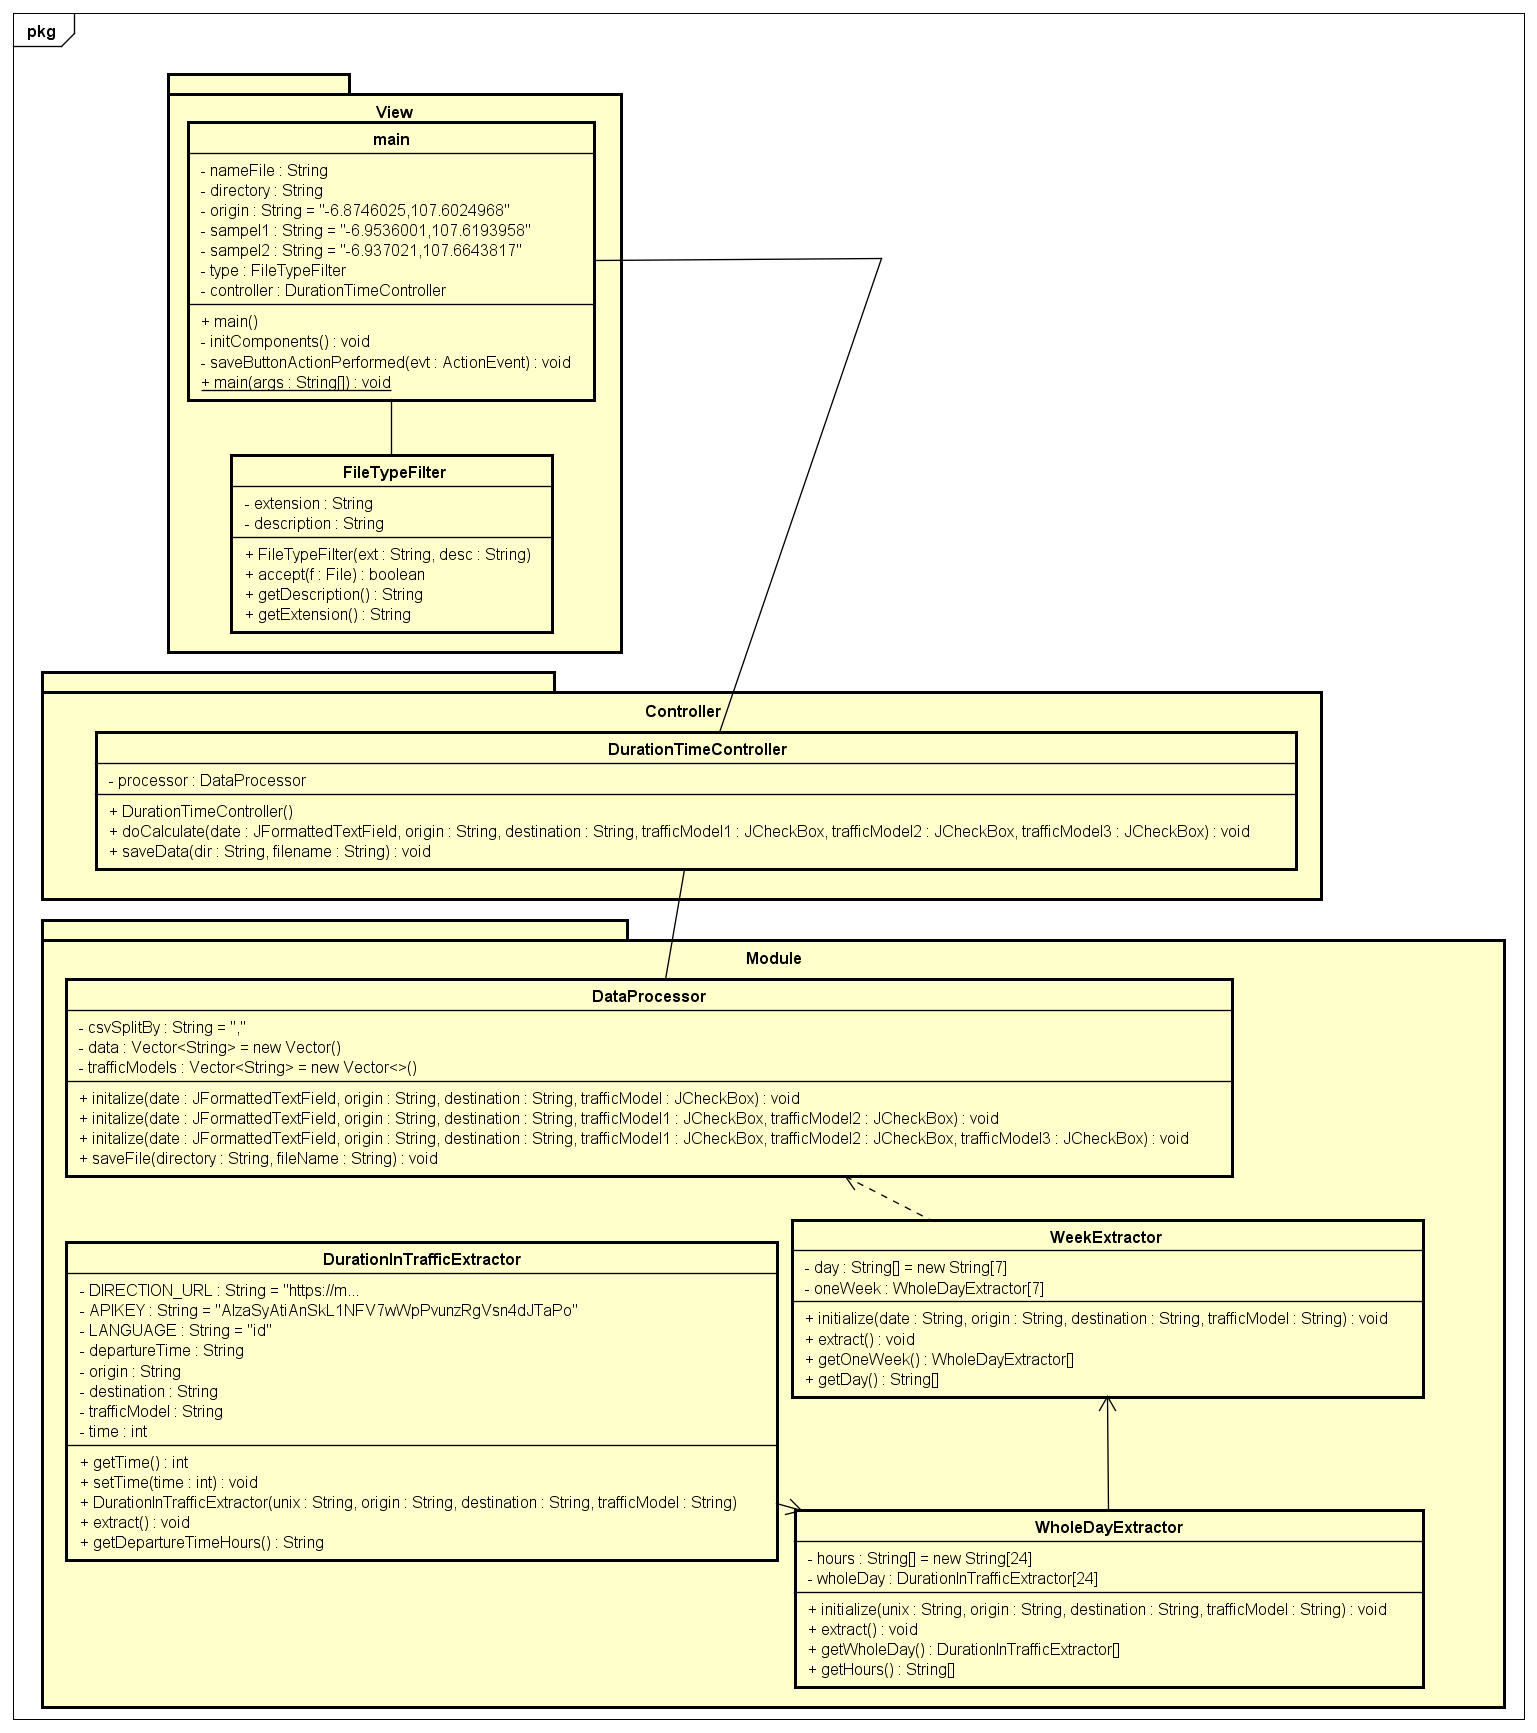
\includegraphics[scale=0.35]{Gambar/classdiagramlengkap.png}
				\caption[Kelas Diagram Rinci]{Kelas Diagram Rinci}
				\label{fig:kelasdiagramrinci}	
			\end{figure}
			
\section{Perancangan Antarmuka}
\label{sec:perancanganantarmuka}

Untuk memenuhi kebutuhan interaksi antara pengguna dengan sistem, maka dirancanglah sebuah antarmuka dari perangkat lunak Analisis Waktu Tempuh Kota Bandun. Rancangan antarmuka dibagi menjadi dua antarmuka antara lain:
\begin{enumerate}
	\item Antarmuka utama.
	
	Antarmuka ini adalah antarmuka utama dari perangkat lunak. Komponen antarmuka ini terdiri dari dua buah \textit{radio button}, \textit{date picker}, tiga buah \textit{check box}, dan sebuah tombol \textit{save} seperti yang ditunjukkan pada Gambar \ref{fig:antarmukautama}. Untuk dapat menyimpan data yang sudah diolah pengguna perlu melakukan input dan memilih sesuai dengan pilihan yang ada di antarmuka yang sesuai kemudian menekan tombol \textit{save}. Jika berhasil pengguna akan diarahkan ke aplikasi Microsoft Excel yang berisikan data-data yang telah didapat.
	
	\begin{figure}[H]
				\centering		
				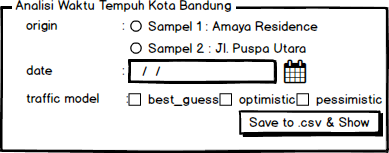
\includegraphics[scale=0.7]{Gambar/Antarmukautama.png}
				\caption[Antarmuka Utama]{Antarmuka Utama}
				\label{fig:antarmukautama}	
			\end{figure}
	
	\item Antarmuka \textit{file chooser}.
	
	Antarmuka ini adalah antarmuka untuk menentukan \textit{directory} penyimpanan file dan menentukan nama file yang akan disimpan. Komponen antarmuka ini seperti yang ditunjukkan pada Gambar \ref{fig:antarmukafilechooser}..
	
	\begin{figure}[H]
				\centering		
				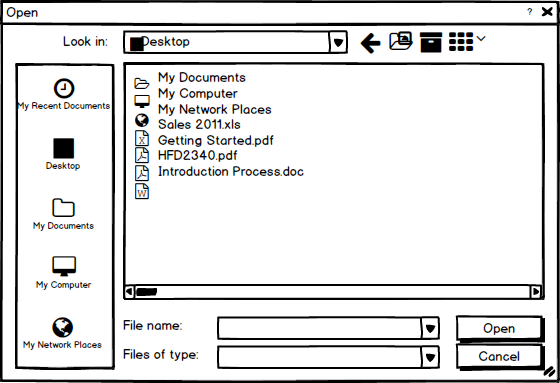
\includegraphics[scale=0.5]{Gambar/WindowsOpenFileDialog.png}
				\caption[Antarmuka \textit{File Chooser}]{Antarmuka \textit{File Chooser}}
				\label{fig:antarmukafilechooser}	
			\end{figure}

\end{enumerate}